\documentclass[12pt]{article}
\usepackage{hyperref}
\usepackage{amsmath}
\usepackage{amsfonts}
\usepackage{amssymb}
\usepackage{graphicx}
\usepackage{caption}
\usepackage{enumerate}
\usepackage{booktabs}

\title{\Huge\textbf{CS215 Assignment 3}}
\author{\Large\textbf{ Group Members :} \\ \\ 
    \large B.Abhinav  23B1018 \\ \\ 
    \large G.Abhiram  23B1084 \\ \\
    \large U.Sai Likhith 23B1058 
} 
\date{\today}
\counterwithin*{equation}{subsection}

\begin{document}



\pagenumbering{arabic}
\maketitle
\newpage

\tableofcontents
\newpage

%%%%%%%%%%%%%%%%%%%%%%%% Question 1 %%%%%%%%%%%%%%%%%%%%%%
\section{Finding optimal bandwidth}
\subsection{Part 1}
\textbf{Solution : } \\
\textbf{a.)} \\ 
We have a data set ${X_1,X_2,\dots,X_n}$,  and we aim to minimize $\hat{J}(h)$ to obtain the optimal h. Given $\hat{p_j}$ is the estimated probability that a 
point falls in the $j^{th}$ bin i.e. $\hat{p_j}=\frac{v_j}{n}$ where $v_{j}$ is the number of points that fall in the $j^{th}$ bin.
We will compute the first term in $\hat{J}(h)$ now that is $\int \hat{f}(x)^2dx$ .
\begin{equation}
    \hat{f}(x)\ =\ \sum_{j=1}^{m}\frac{\hat{p_j}}{h}\mathbb{I}[x \in B_j]
\end{equation}
The above is the histogram estimate.
\begin{equation*}
\begin{split}
    \int \hat{f}(x)^2dx &= \sum_{j=1}^{m}\int_{B_j}^{}\left(\sum_{k=1}^{m}\frac{\hat{p_k}}{h}\mathbb{I}[x \in B_k]\right)^2dx  \\
                        &= \sum_{j=1}^{m}\int_{B_j}^{}\left( \frac{\hat{p_j}}{h}\right)^2 dx \\
                        &= \sum_{j=1}^{m}\int_{B_j}^{}\frac{v_j^2}{n^2h^2}dx = \sum_{j=1}^{m}\frac{v_j^2}{n^2h^2}h 
\end{split}
\end{equation*}
Because all bins are of equal length $h$. Hence we proved that 
\begin{equation}
    \boxed{\int \hat{f}(x)^2dx\ =\  \frac{1}{n^2h}\sum_{j=1}^{m}v_j^2 }
\end{equation}
\\
\textbf{b.)} \\
Lets now compute $\sum_{i=1}^{n}\hat{f}_{(-i)}(X_i)$ and prove that it is equivalent to 
\[\frac{1}{(n-1)h}\sum_{j=1}^{m}(v_j^2-v_j)\]
where $\hat{f}_{(-i)}$ is the histogram estimator after removing $i^{th}$ observation.
We have $\hat{f}_{(-i)}(X_i)\ =\ \sum_{j=1}^{m}\frac{\hat{p_j}}{h}\mathbb{I}[X_i \in B_j]\ =\ \sum_{j=1}^{m}\frac{v_j}{(n-1)h}\mathbb{I}[X_i \in B_j]$ where $v_j$ is the new updated one after removing $X_i$.
If $X_i \in B_j$ this simplifies to $\frac{v_j-1}{(n-1)h}$.
Let $S_j\ =\ \{X_i\ ,1\le i \le n|\ X_i \in B_j\}$
We have 
\begin{equation*}
\begin{split}
    \sum_{i=1}^{n}\hat{f}_{(-i)}(X_i) &=  \sum_{j=1}^{m}\sum_{x \in S_j}^{}\hat{f}_{(-i)}(x) \\
                                      &=  \sum_{j=1}^{m}\sum_{x \in S_j}^{}\frac{v_j-1}{(n-1)h} \ where\ |S_j|=v_j\\
                                      &=  \sum_{j=1}^{m}\frac{v_j(v_j-1)}{(n-1)h}
\end{split}
\end{equation*}
Therefore we proved that: 
\begin{equation}
    \boxed{\sum_{i=1}^{n}\hat{f}_{(-i)}(X_i)\ =\ \frac{1}{(n-1)h}\sum_{j=1}^{m}(v_j^2-v_j)}
\end{equation}

\subsection{Part 2}
\textbf{Solution: } \\
a.) The following are the estimated probabilities $\hat{p}_{j}$ for all bins with total number of bins $m=10$ rounded off to 4 decimals.
\begin{table}[h]
    \centering
    \begin{tabular}{@{}cc@{}}
        \toprule
        \textbf{Bin(j)} & \textbf{Probability ($\hat{p}_j$)} \\ \midrule
        1  & 0.2059 \\
        2  & 0.4882 \\
        3  & 0.0471 \\
        4  & 0.0412 \\
        5  & 0.1353 \\
        6  & 0.0588 \\
        7  & 0.0059 \\
        8  & 0.0000 \\
        9  & 0.0118 \\
        10 & 0.0059 \\ \bottomrule
    \end{tabular}
    \caption{Estimated probabilities for each bin}
    \label{tab:probabilities}
\end{table} \\
b.) The histogram is underfit as it has been oversmoothed due to too few bins,
which results in a loss of important details. This underfitting prevents the histogram from 
accurately representing the underlying distribution of the data ie has higher loss function. We need to increase the number of bins
so as to find the optimal bin width ie that which minimizes loss \\
\\
d.) Optimal value of bin width $h^*$ =  0.06835999999999999 and occurs at $m=50$ that is 50 bins.
This was found by minimizing the cross-validation estimator \\
\\
e.)\textbf{Detail and Information Capture}: The histogram with $m=50$ captures significantly more detail than the one with 
$m=10$. While the histogram with $m=10$ appears smooth and oversimplified, the $m=50$ histogram reveals additional features in the data distribution.
\\
\textbf{Peaks and Minima:} The histogram with \( m = 50 \) shows new peaks and minima that are not visible in the \( m = 10 \) histogram. This suggests a more complex structure in the data, indicating the presence of clusters or gaps that might be important for understanding the distribution of distances.


\section{Detecting Anomalous Transactions using KDE}
\subsection{Designing a custom KDE Class}
Check $2.py$
\subsection{Estimating Distribution of Transactions}
The 3D probability density deduced using kernel estimate plot is in next page \\ 
I have used band width = 0.25 and observed 4035 modes. \\
\begin{table}[h]
    \centering
    \begin{tabular}{cc}
    \hline
    \textbf{Bandwidth (h)} & \textbf{Number of Modes} \\ \hline
    0.1 & 5011 \\
    0.25 & 4035 \\
    0.5 & 3298 \\
    1 & 2263 \\ \hline
    \end{tabular}
    \caption{Bandwidth and Number of Modes}
    \label{tab:bandwidth_modes}
    \end{table}
% \begin{minipage}{\linewidth}
%     \begin{center}
%         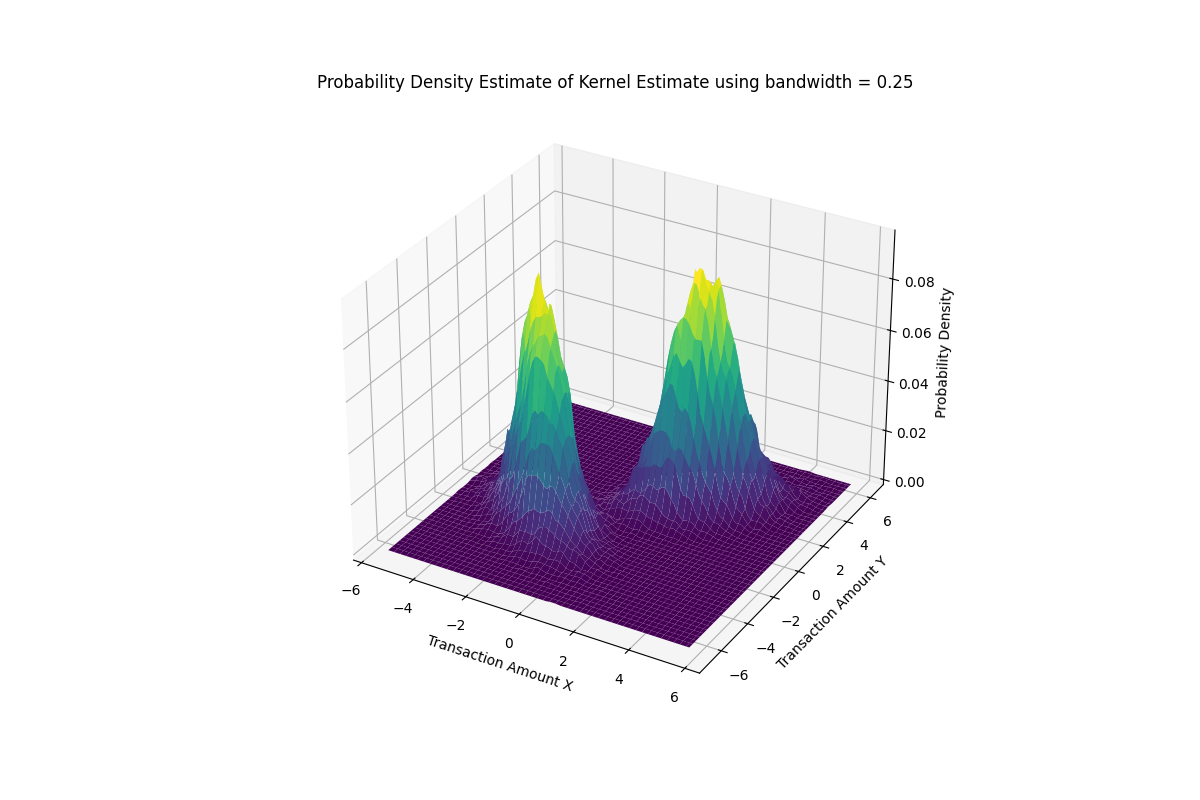
\includegraphics[width=1\textwidth]{images/transaction_distribution.png}
%         \captionof{figure}{3D Probability Density of Transactions}
%     \end{center}
% \end{minipage}
\begin{minipage}{\linewidth}
    \begin{center}
        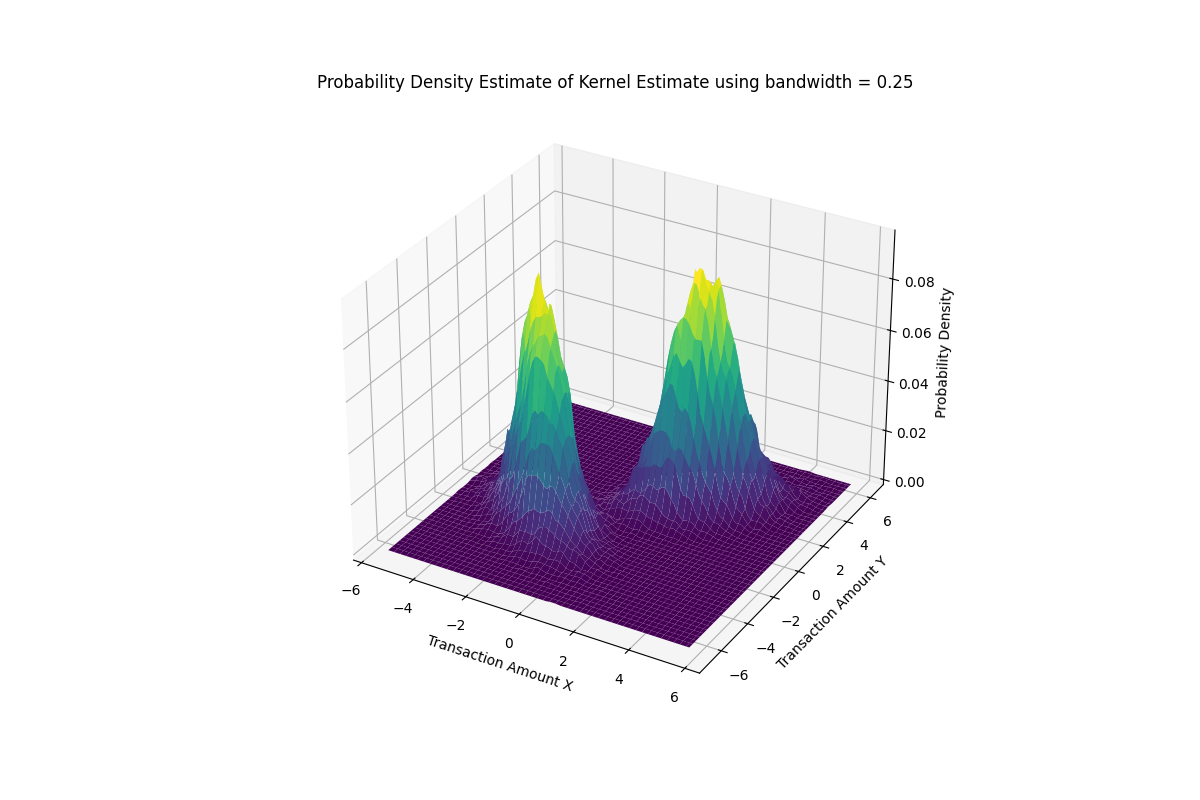
\includegraphics[width=\textwidth]{images/transaction_distribution.png}
        \captionof{figure}{3D Probability Density of Transactions}
    \end{center}
\end{minipage}
\end{document}